\documentclass{article}
\usepackage[utf8]{inputenc}
\usepackage{graphicx}
\usepackage{float}
\usepackage{hyperref}
\usepackage{titling}

\usepackage[scale=0.8, bmargin=2cm, tmargin=2cm, lmargin=3cm, rmargin=3cm]{geometry}

\begin{document}

\title{\textbf{Rapport projet TSMA \\
Classification Audio}}
\author{Guillaume Almyre, Pierre Célor et Antoine Pirrone}



\date{\today}
\pretitle{%
  \begin{center}
  \LARGE
  
\includegraphics[scale=0.3]{assets/ub_logo.jpg}\\[\bigskipamount]
  \vspace{3cm}
}
\posttitle{\end{center}}
\maketitle

\newpage

\section*{Introduction}

Le but de ce projet était d'implémenter un classifieur de musique en utilisant une bibliothèque de machine learning/deep learning de notre choix. Nous avons choisi d'explorer la piste des Réseaux de Neurones, et la bibliothèque que nous avons choisi d'utiliser est \textbf{TensorFlow} en Python, couplée à la bibliothèque \textbf{Librosa} pour l'extraction des features audio.\\

Notre projet s'organise de la façon suivante :

\begin{itemize}
  
\item \textbf{extract.py} : extrait les features (cf partie Choix Techniques) et les sauvegarde. L'extraction de features est très longue (quelques heures pour tout extraire de la base de morceaux de musique fournie), donc nous ne voulions pas le refaire à chaque entrainement.
  
\item \textbf{train.py} : génère le réseau de neurones avec tensorflow et l'entraine. Ce programme prend directement en entrée les fichiers de features extraits par \textbf{extract.py}

\item \textbf{sample.py} : programme pour échantillonner un modèle entrainé, évalue la classe d'un ou plusieurs fichier audio passé en paramètres (sauvegarde au passage les features extraites, pour gagner du temps plus tard)

\item \textbf{sampleFromFeatures.py} : même chose que \textbf{sample.py} mais à partir de fichiers de features précedemment sauvegardées

\item \textbf{reformat.sh} : petit script pour formater la sortie de \textbf{sampleFromFeatures.py} dans le bon format pour le challenge kaggle
  
\end{itemize}

\section*{Choix des descripteurs}

Dans \textbf{extract.py}, on extrait un certain nombre de features (descripteurs) par morceau, nous extrayons les features suivantes grâce à \textbf{Librosa} :

\begin{itemize}

  \item \textbf{mfcc} : Mel-frequency cepstral coefficients 
  \item \textbf{chroma\_stft} : "Chromagramme" de la  Short Term Fourier Transform
  \item \textbf{melspectrogram} : Spectrogramme sur une échelle de Mel
  \item \textbf{spectral\_contrast} : contraste spectral (spectral contrast)
  \item \textbf{tonnez} : centroïde tonal (tonal centroid)
    
\end{itemize}




\section*{Description du modèle}



\section*{Résultats}


\begin{figure}[h]
  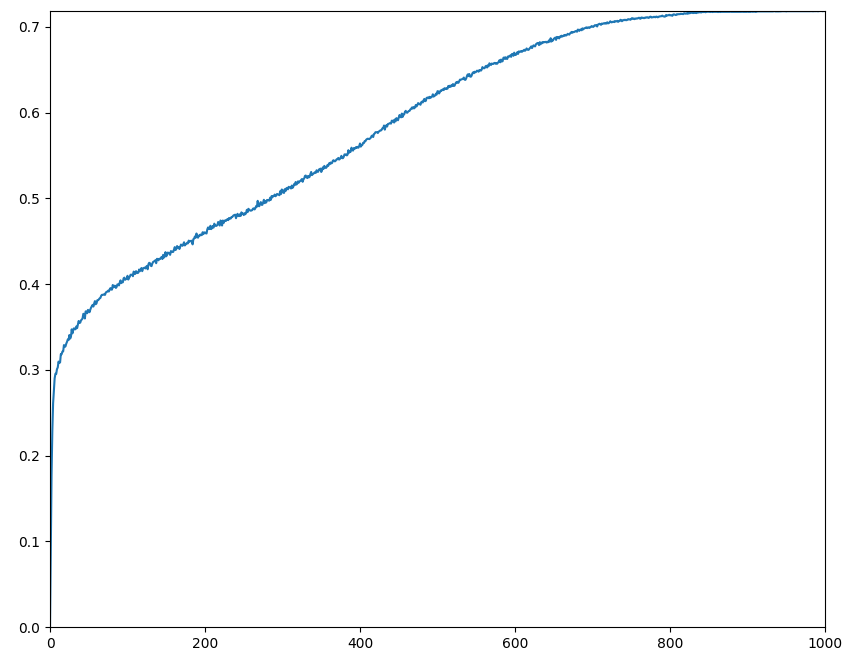
\includegraphics[scale=0.264]{assets/acc}
  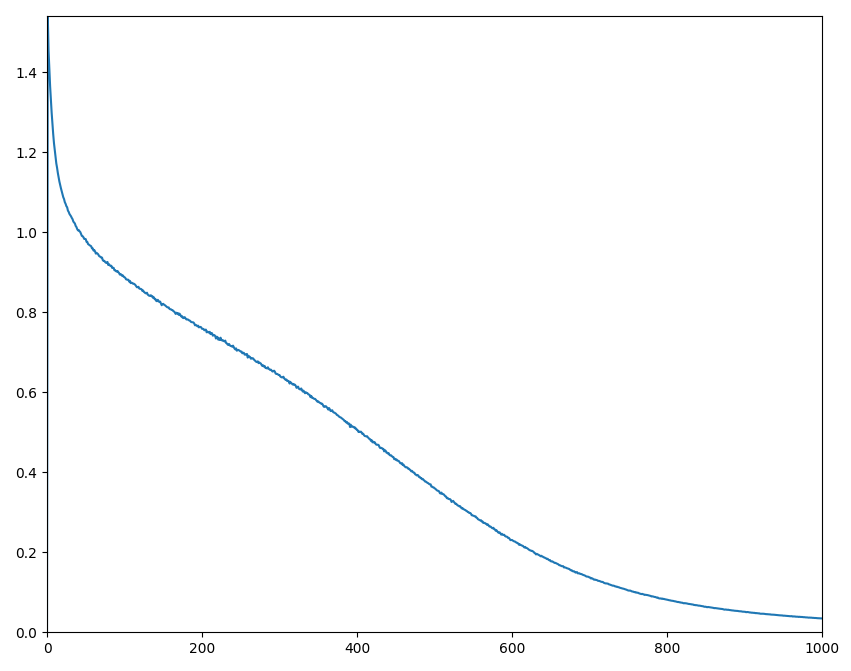
\includegraphics[scale=0.265]{assets/loss}
  
  \caption{À gauche, la précision (accuracy) du modèle pendant l'entrainement. À droite, son erreur (cost)}
  \label{acc_los}
\end{figure}

\section*{Améliorations possibles}

\section*{Conclusion}


\end{document}
